% !TEX encoding = UTF-8 Unicode
%!TEX root = ../Main/thesis.tex
% !TEX spellcheck = en-US
%%=========================================
\documentclass[../Main/thesis.tex]{subfiles}
\begin{document}
\chapter{Prototype Evaluation}
\label{ch:evaluation}
This chapter describes the final evaluation of the FireTracker system.
The evaluation was done with representatives from Øygarden Fire and Rescue, at their offices and training facilities in Ågotnes.

\section{Preparations}
As a preparation for the evaluation all the beacons were labeled with a number that matched the name they were given in the exercise management tool. 
The transmitting signal strength of all the beacons were set to the lowest possible value, and all of them were turned on.
The two Android devices, and a backup device was fully charged.

\begin{figure}[h]
	\centering
	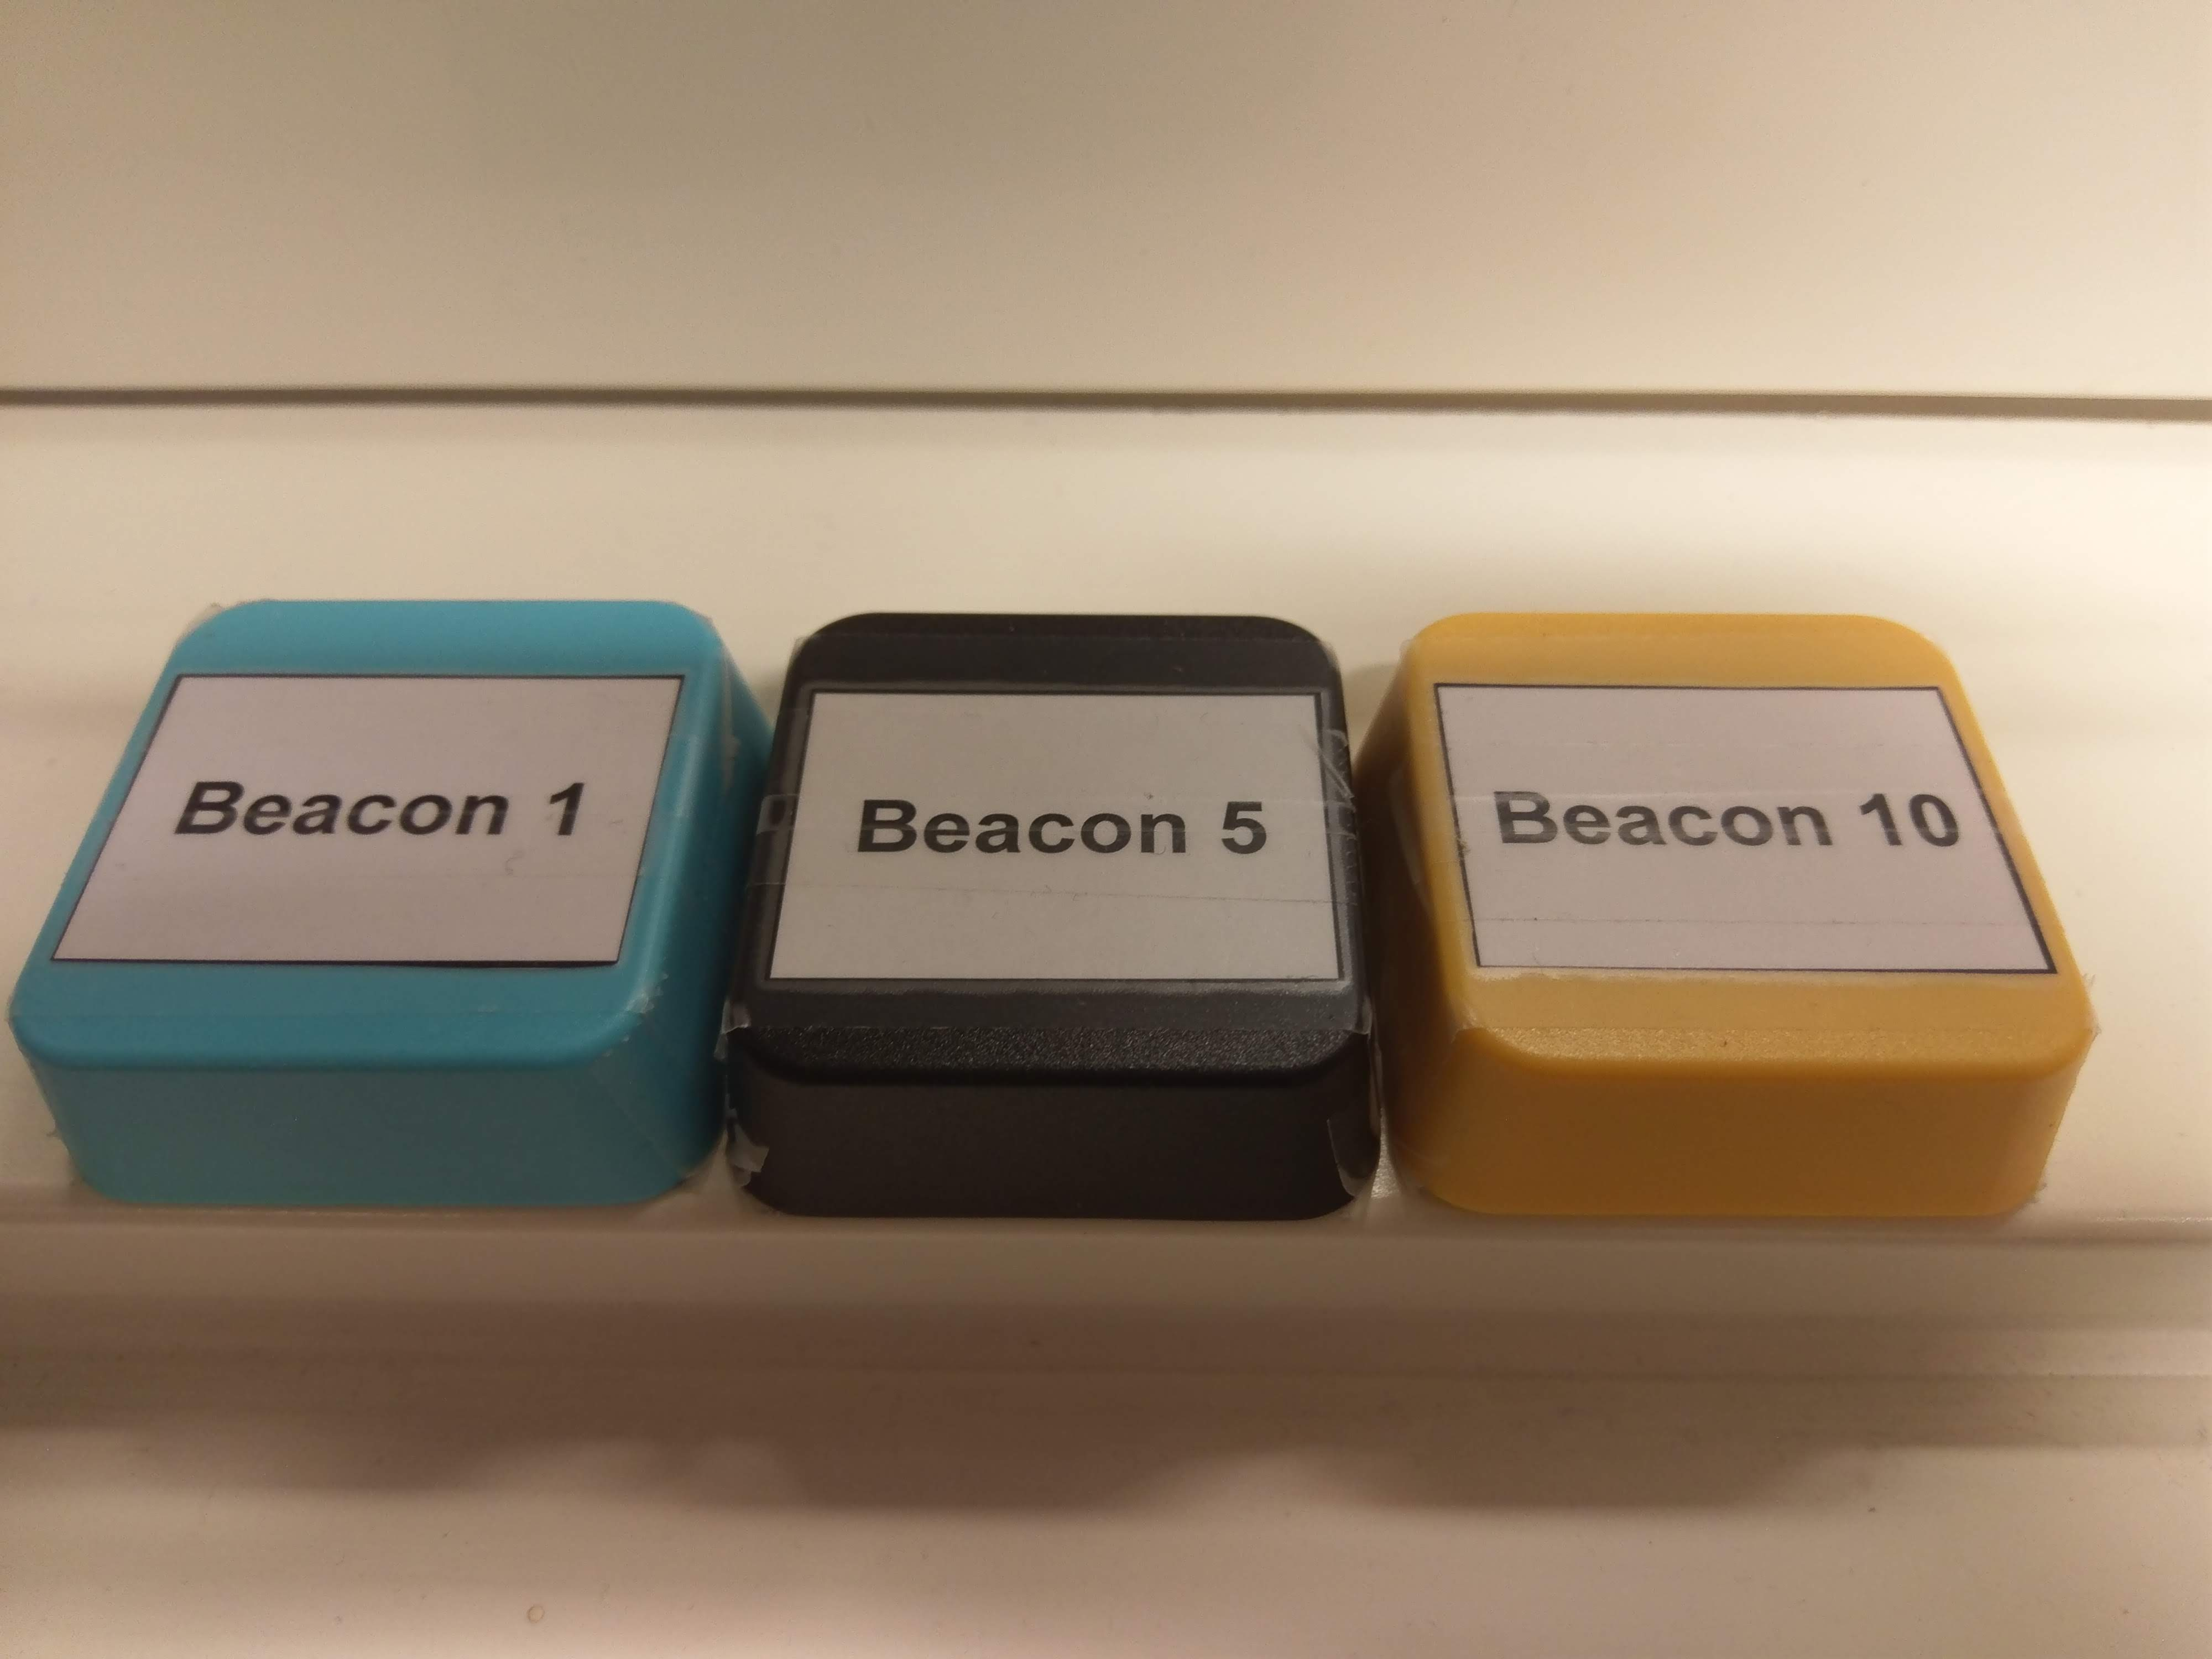
\includegraphics[width=\textwidth]{../fig/beacons}
	\caption{Numbered BLE beacons}
	\label{fig:beacons}
\end{figure}
\section{Test of FireTracker}

\begin{figure}[h]
	\centering
	\begin{subfigure}{0.45\textwidth}
		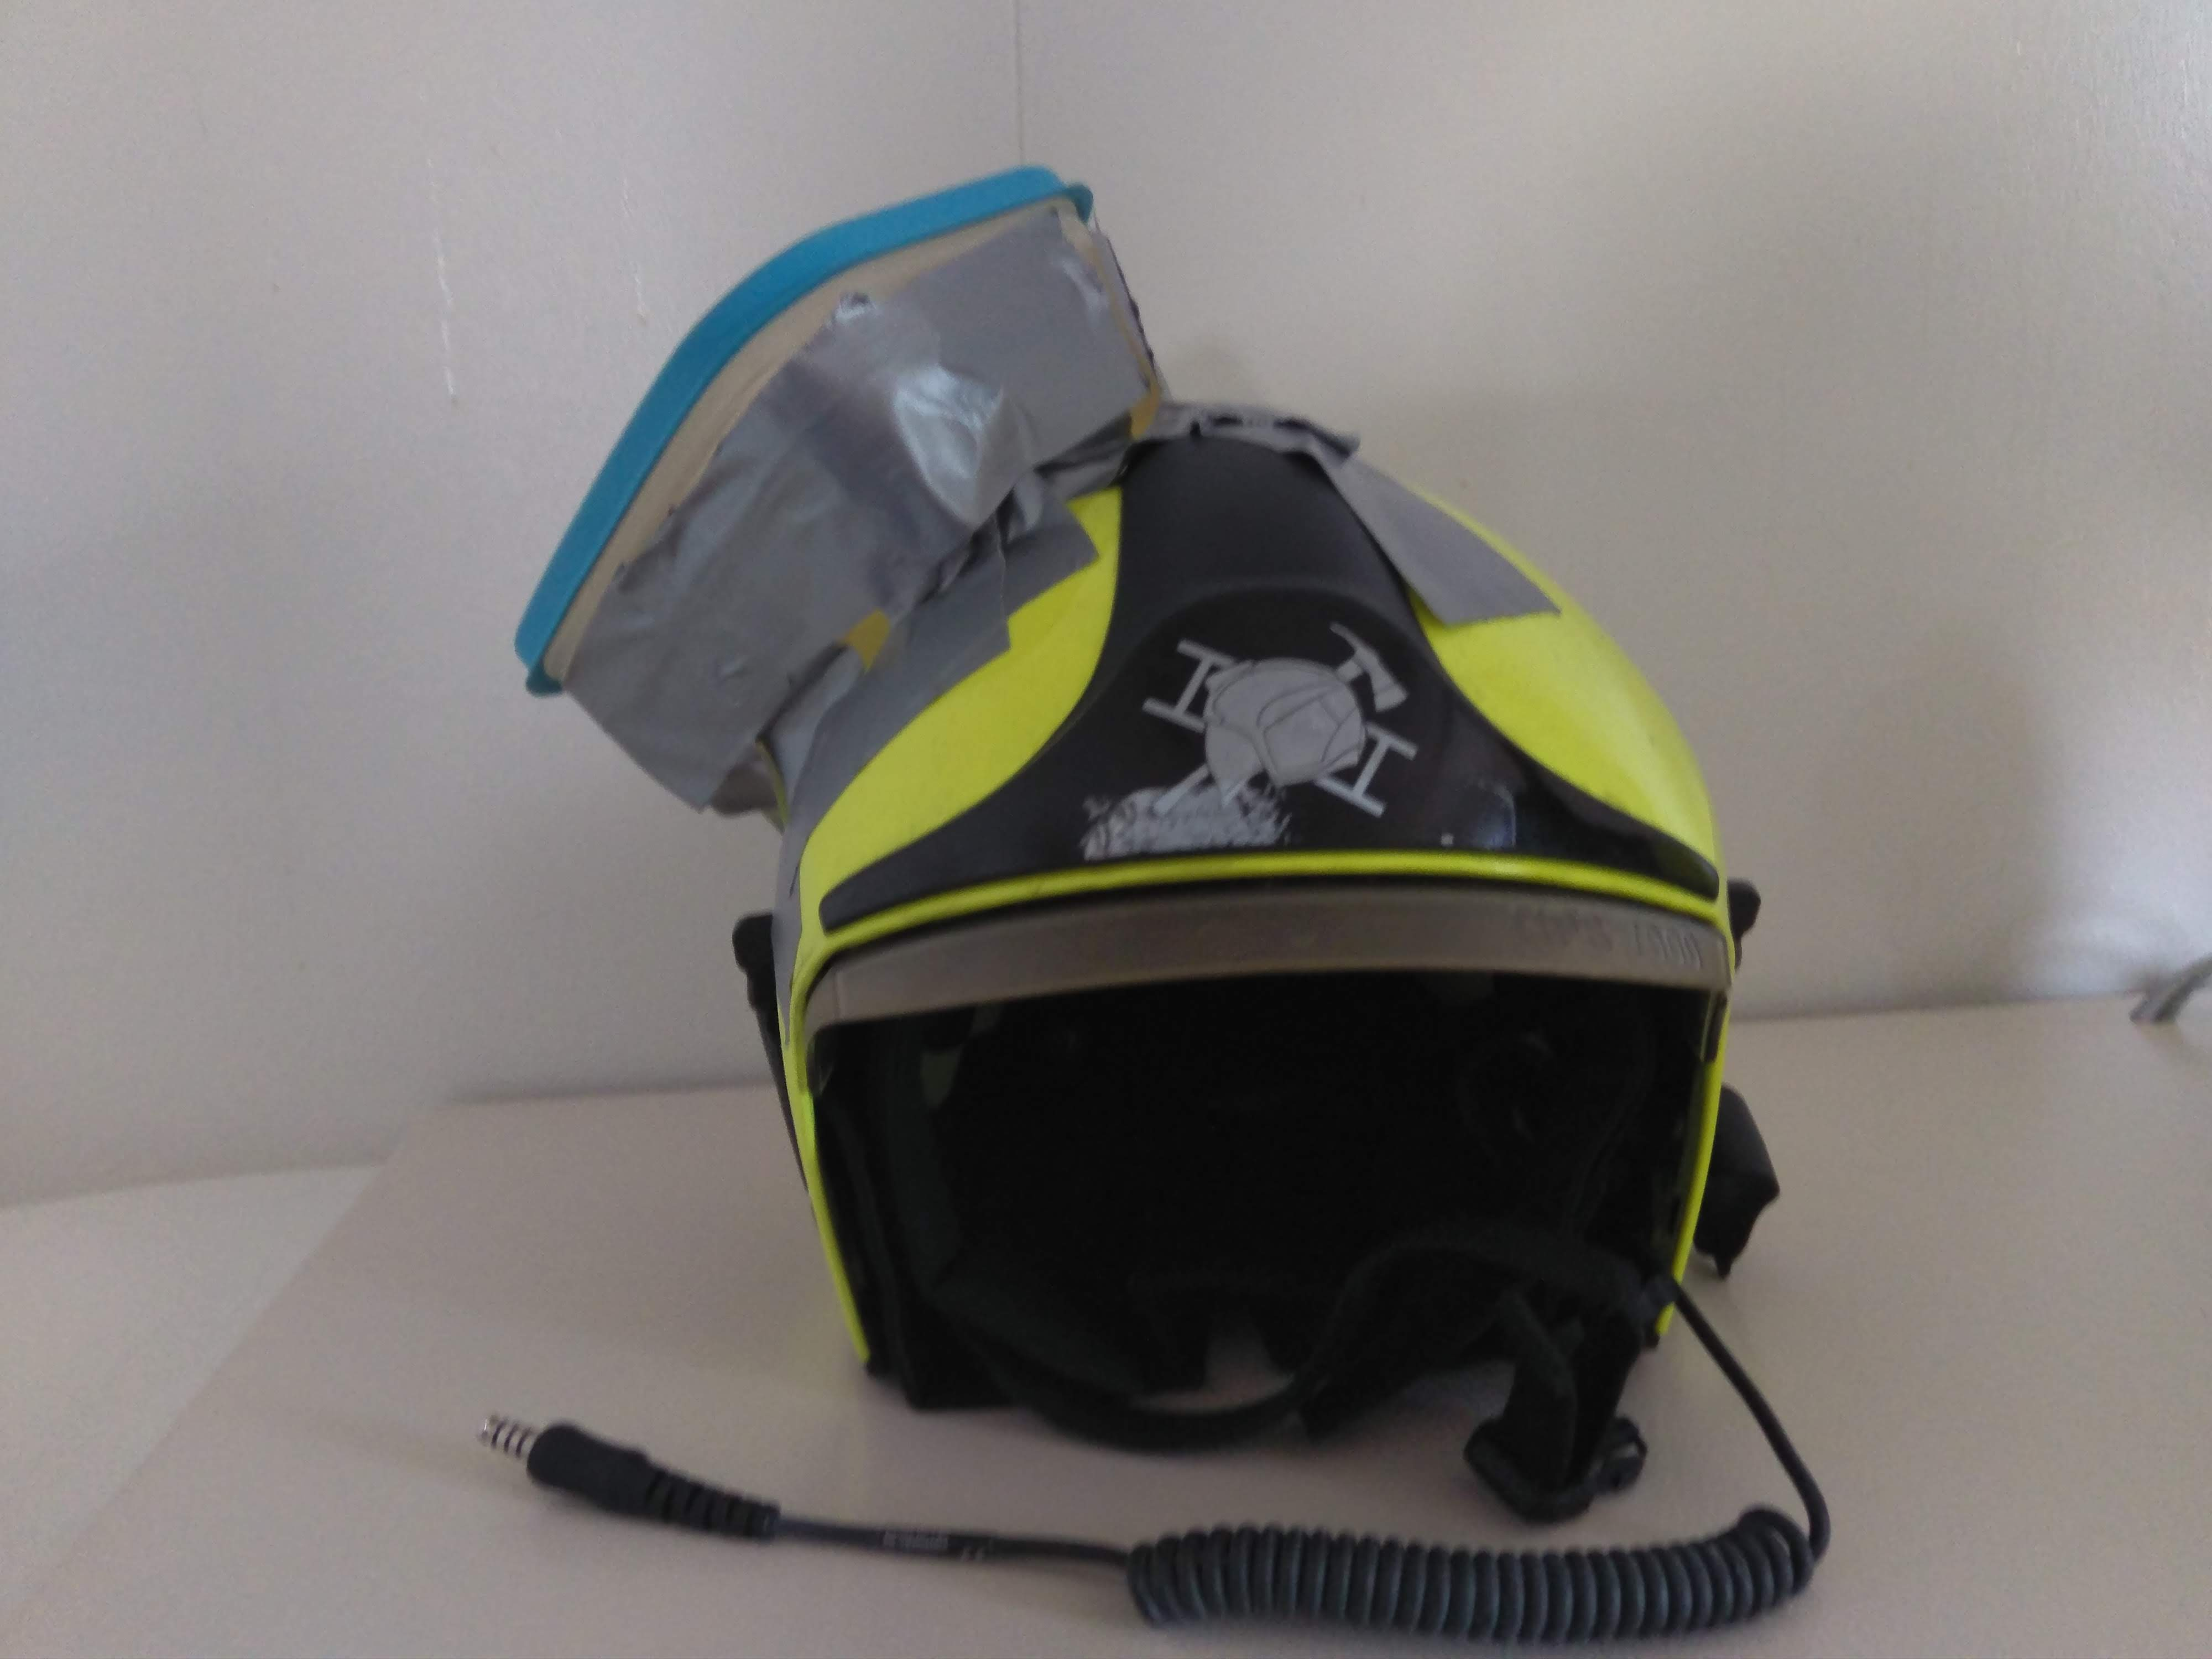
\includegraphics[width=\textwidth]{../fig/helmet-front}
		\caption{Front of helmet}
		\label{fig:eval-helmet-front}
	\end{subfigure}
	\begin{subfigure}{0.45\textwidth}
		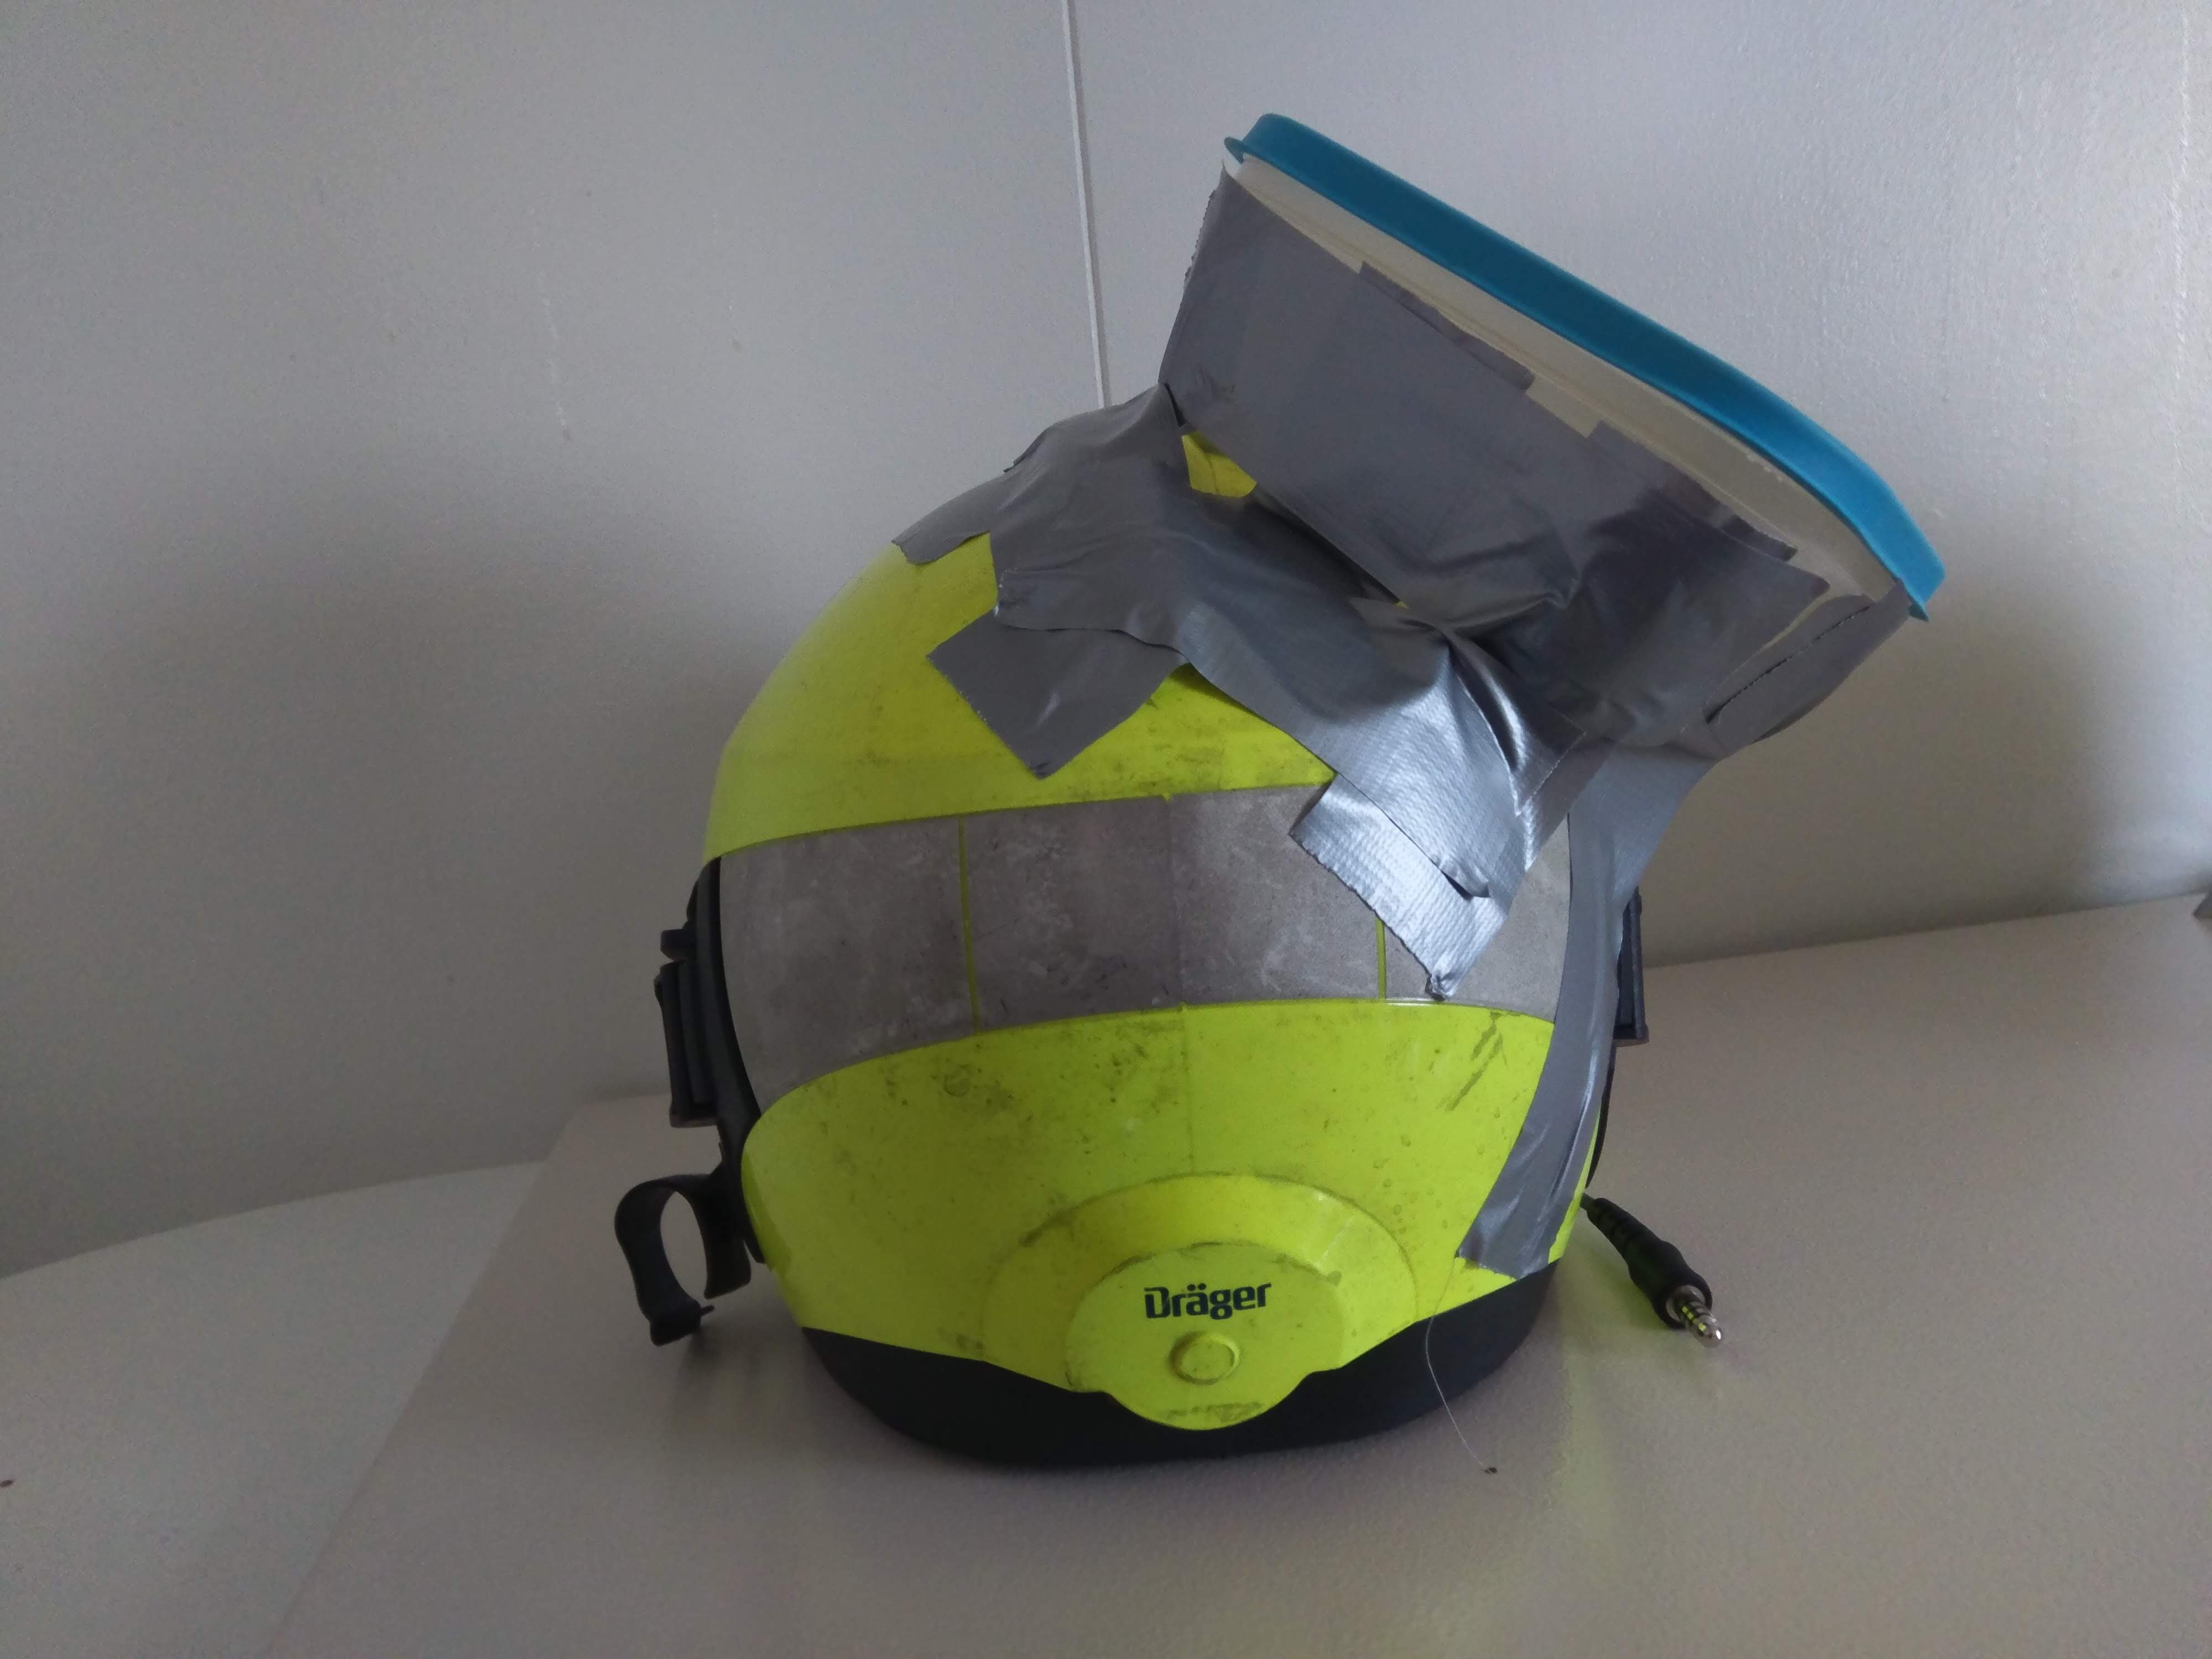
\includegraphics[width=\textwidth]{../fig/helmet-back}
		\caption{Backside of helmet}
		\label{fig:eval-helmet-back}
	\end{subfigure}
	\begin{subfigure}{0.45\textwidth}
		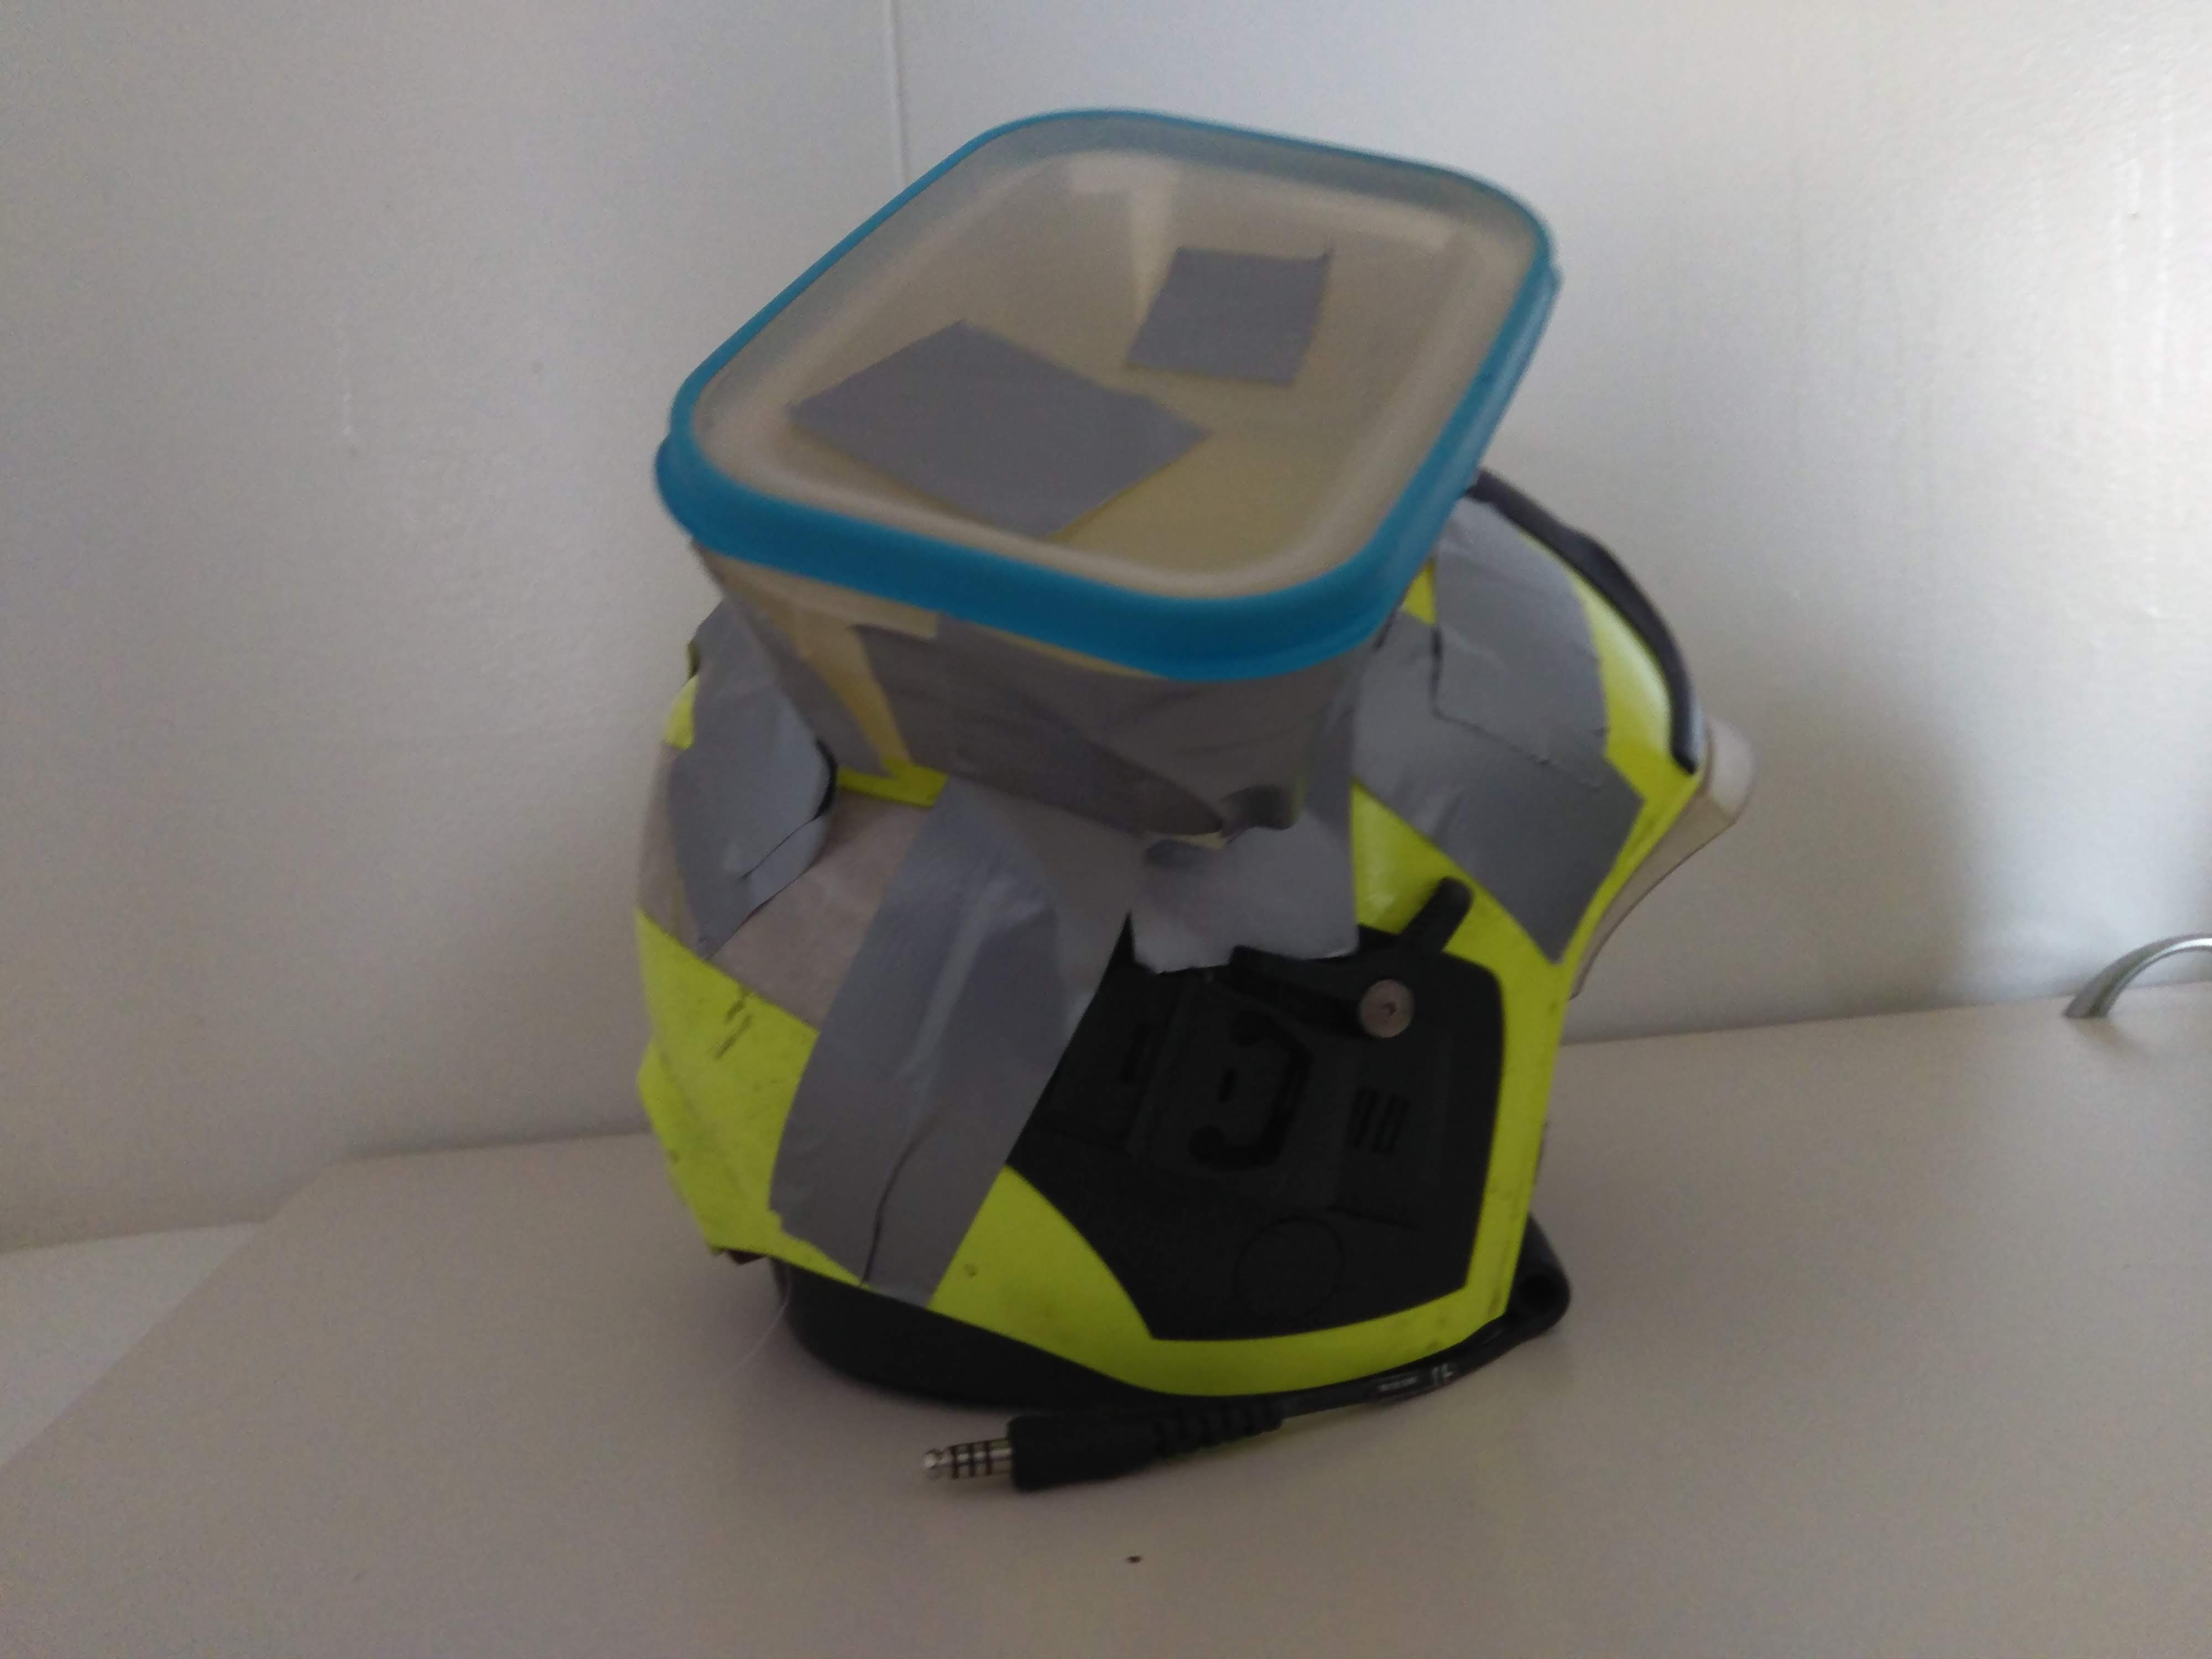
\includegraphics[width=\textwidth]{../fig/helmet-right}
		\caption{Right side of helmet}
		\label{fig:eval-helmet-right}
	\end{subfigure}
	\begin{subfigure}{0.45\textwidth}
		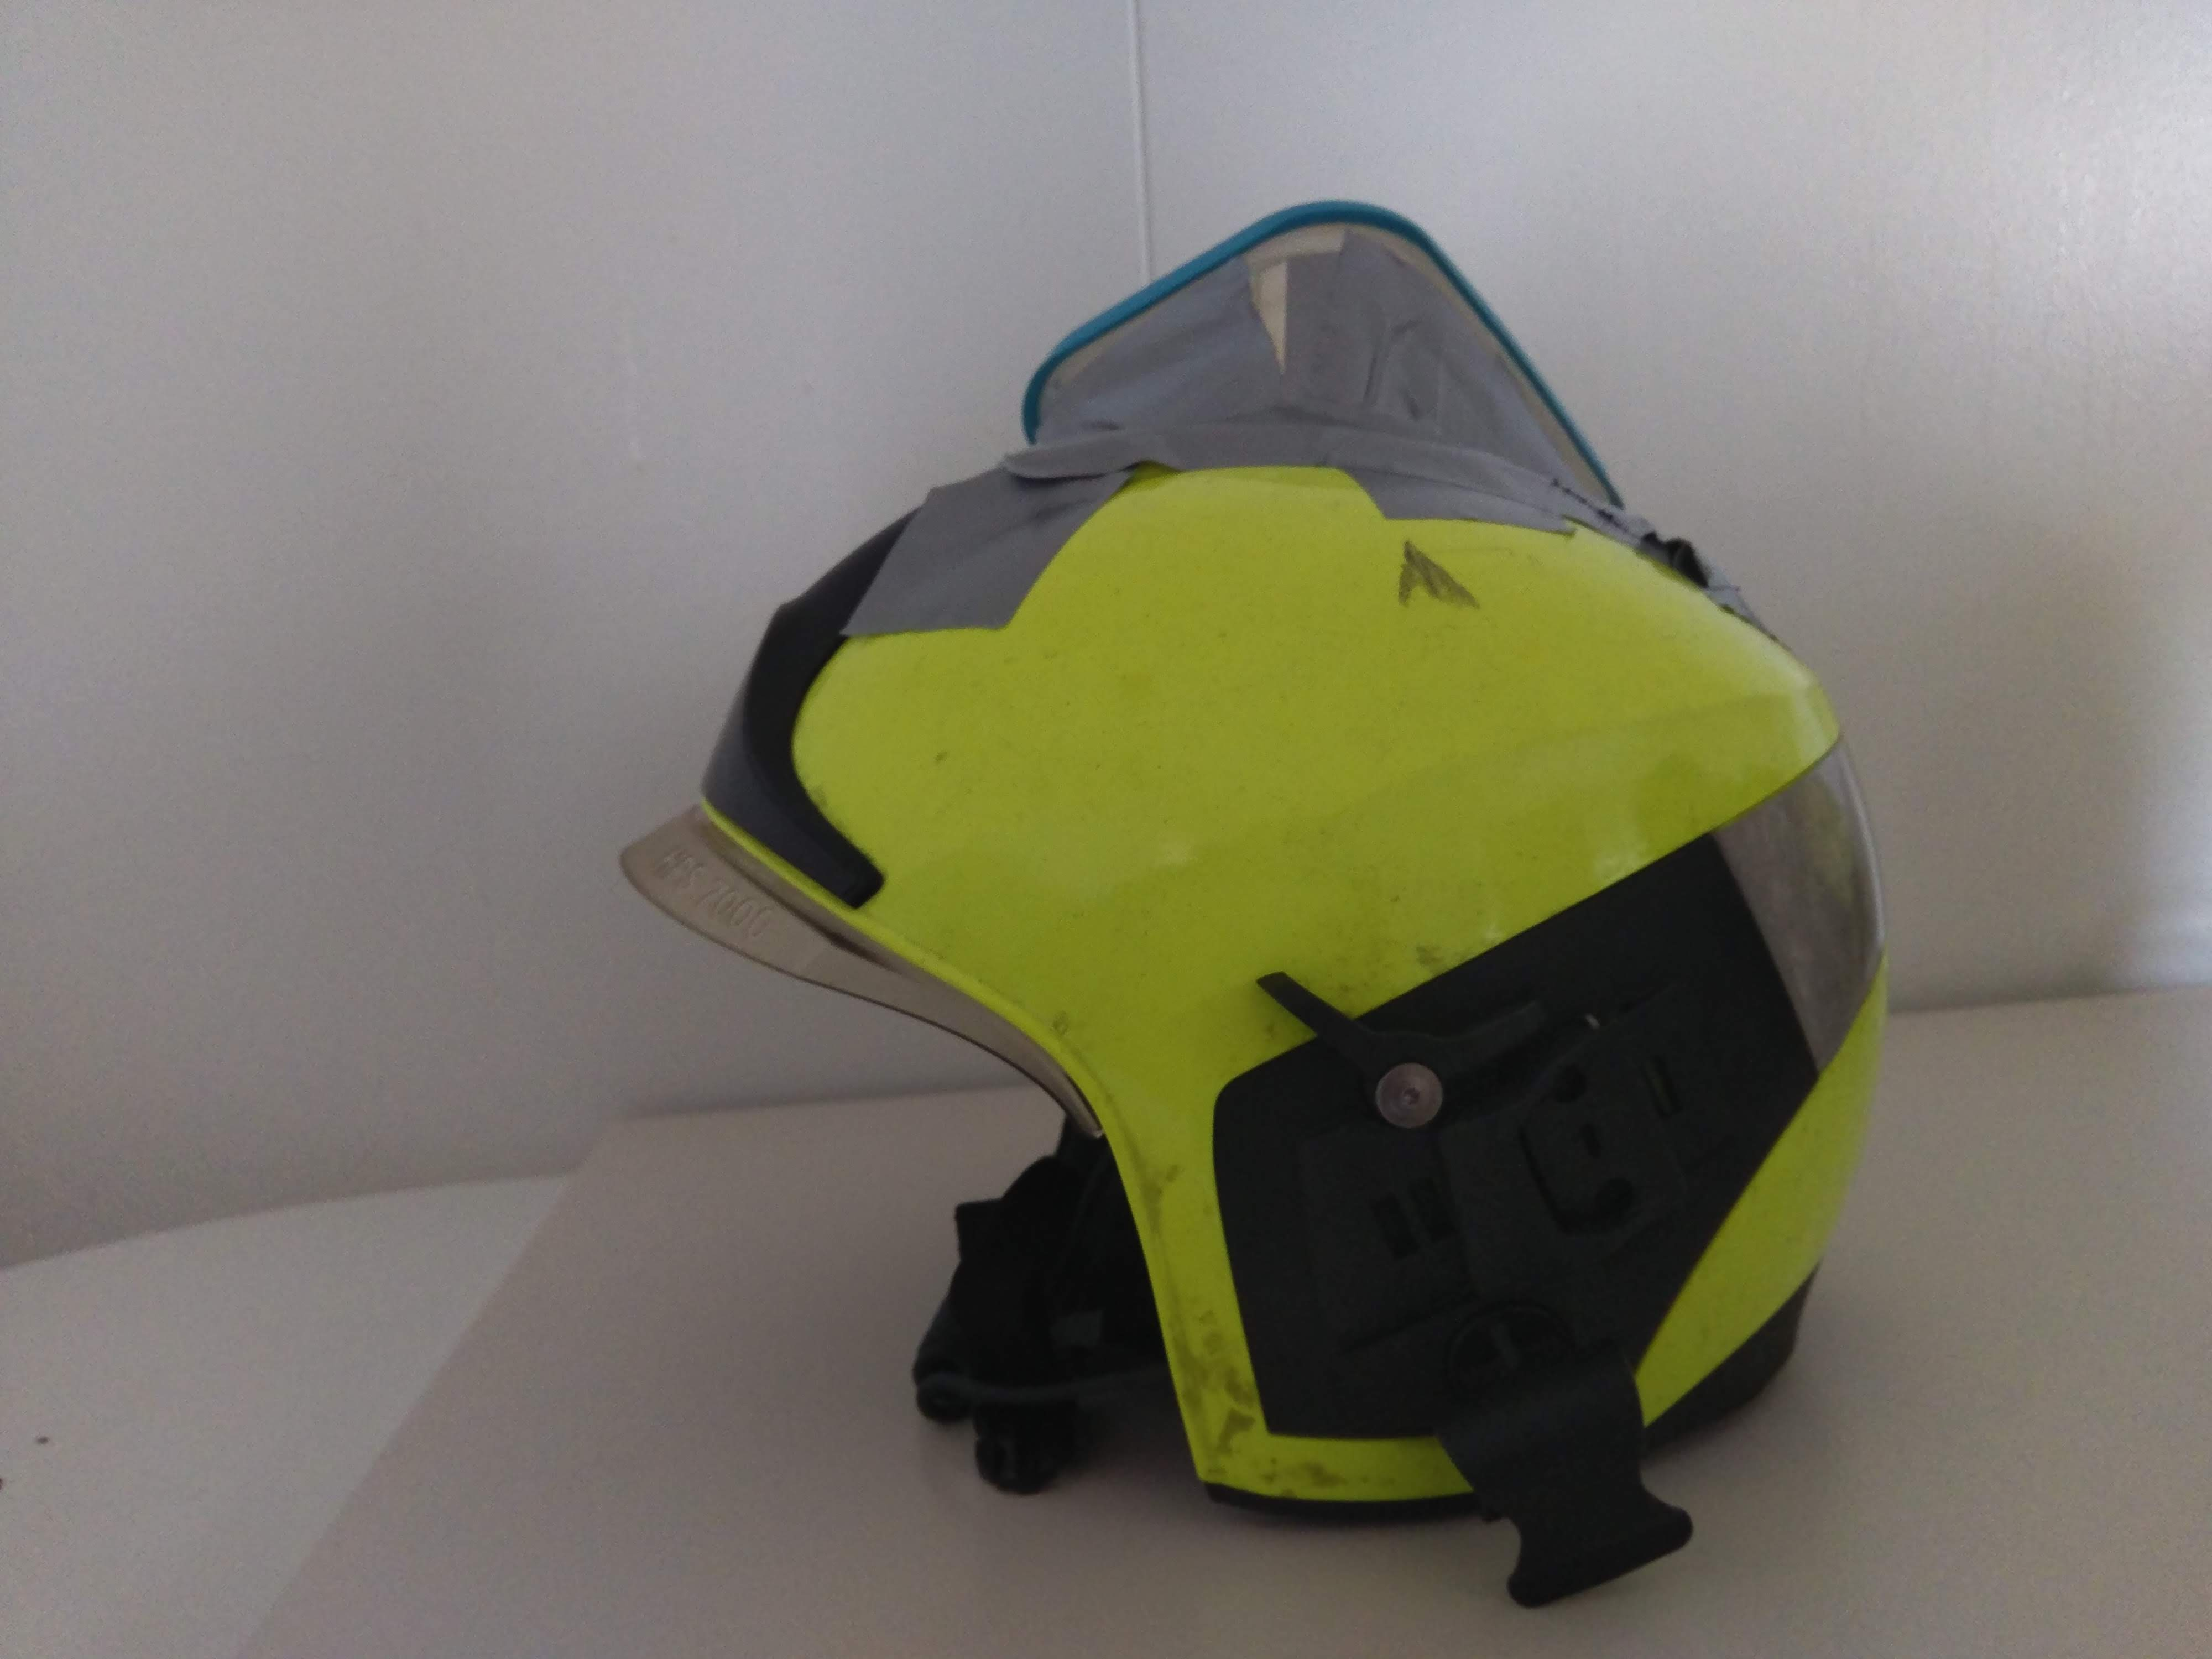
\includegraphics[width=\textwidth]{../fig/helmet-left}
		\caption{Left side of helmet}
		\label{fig:eval-helmet-left}
	\end{subfigure}
	\caption{Plastic box for smartphone attached to helmet}
	\label{fig:eval-helmet}
\end{figure}

\begin{figure}[h]
	\centering
	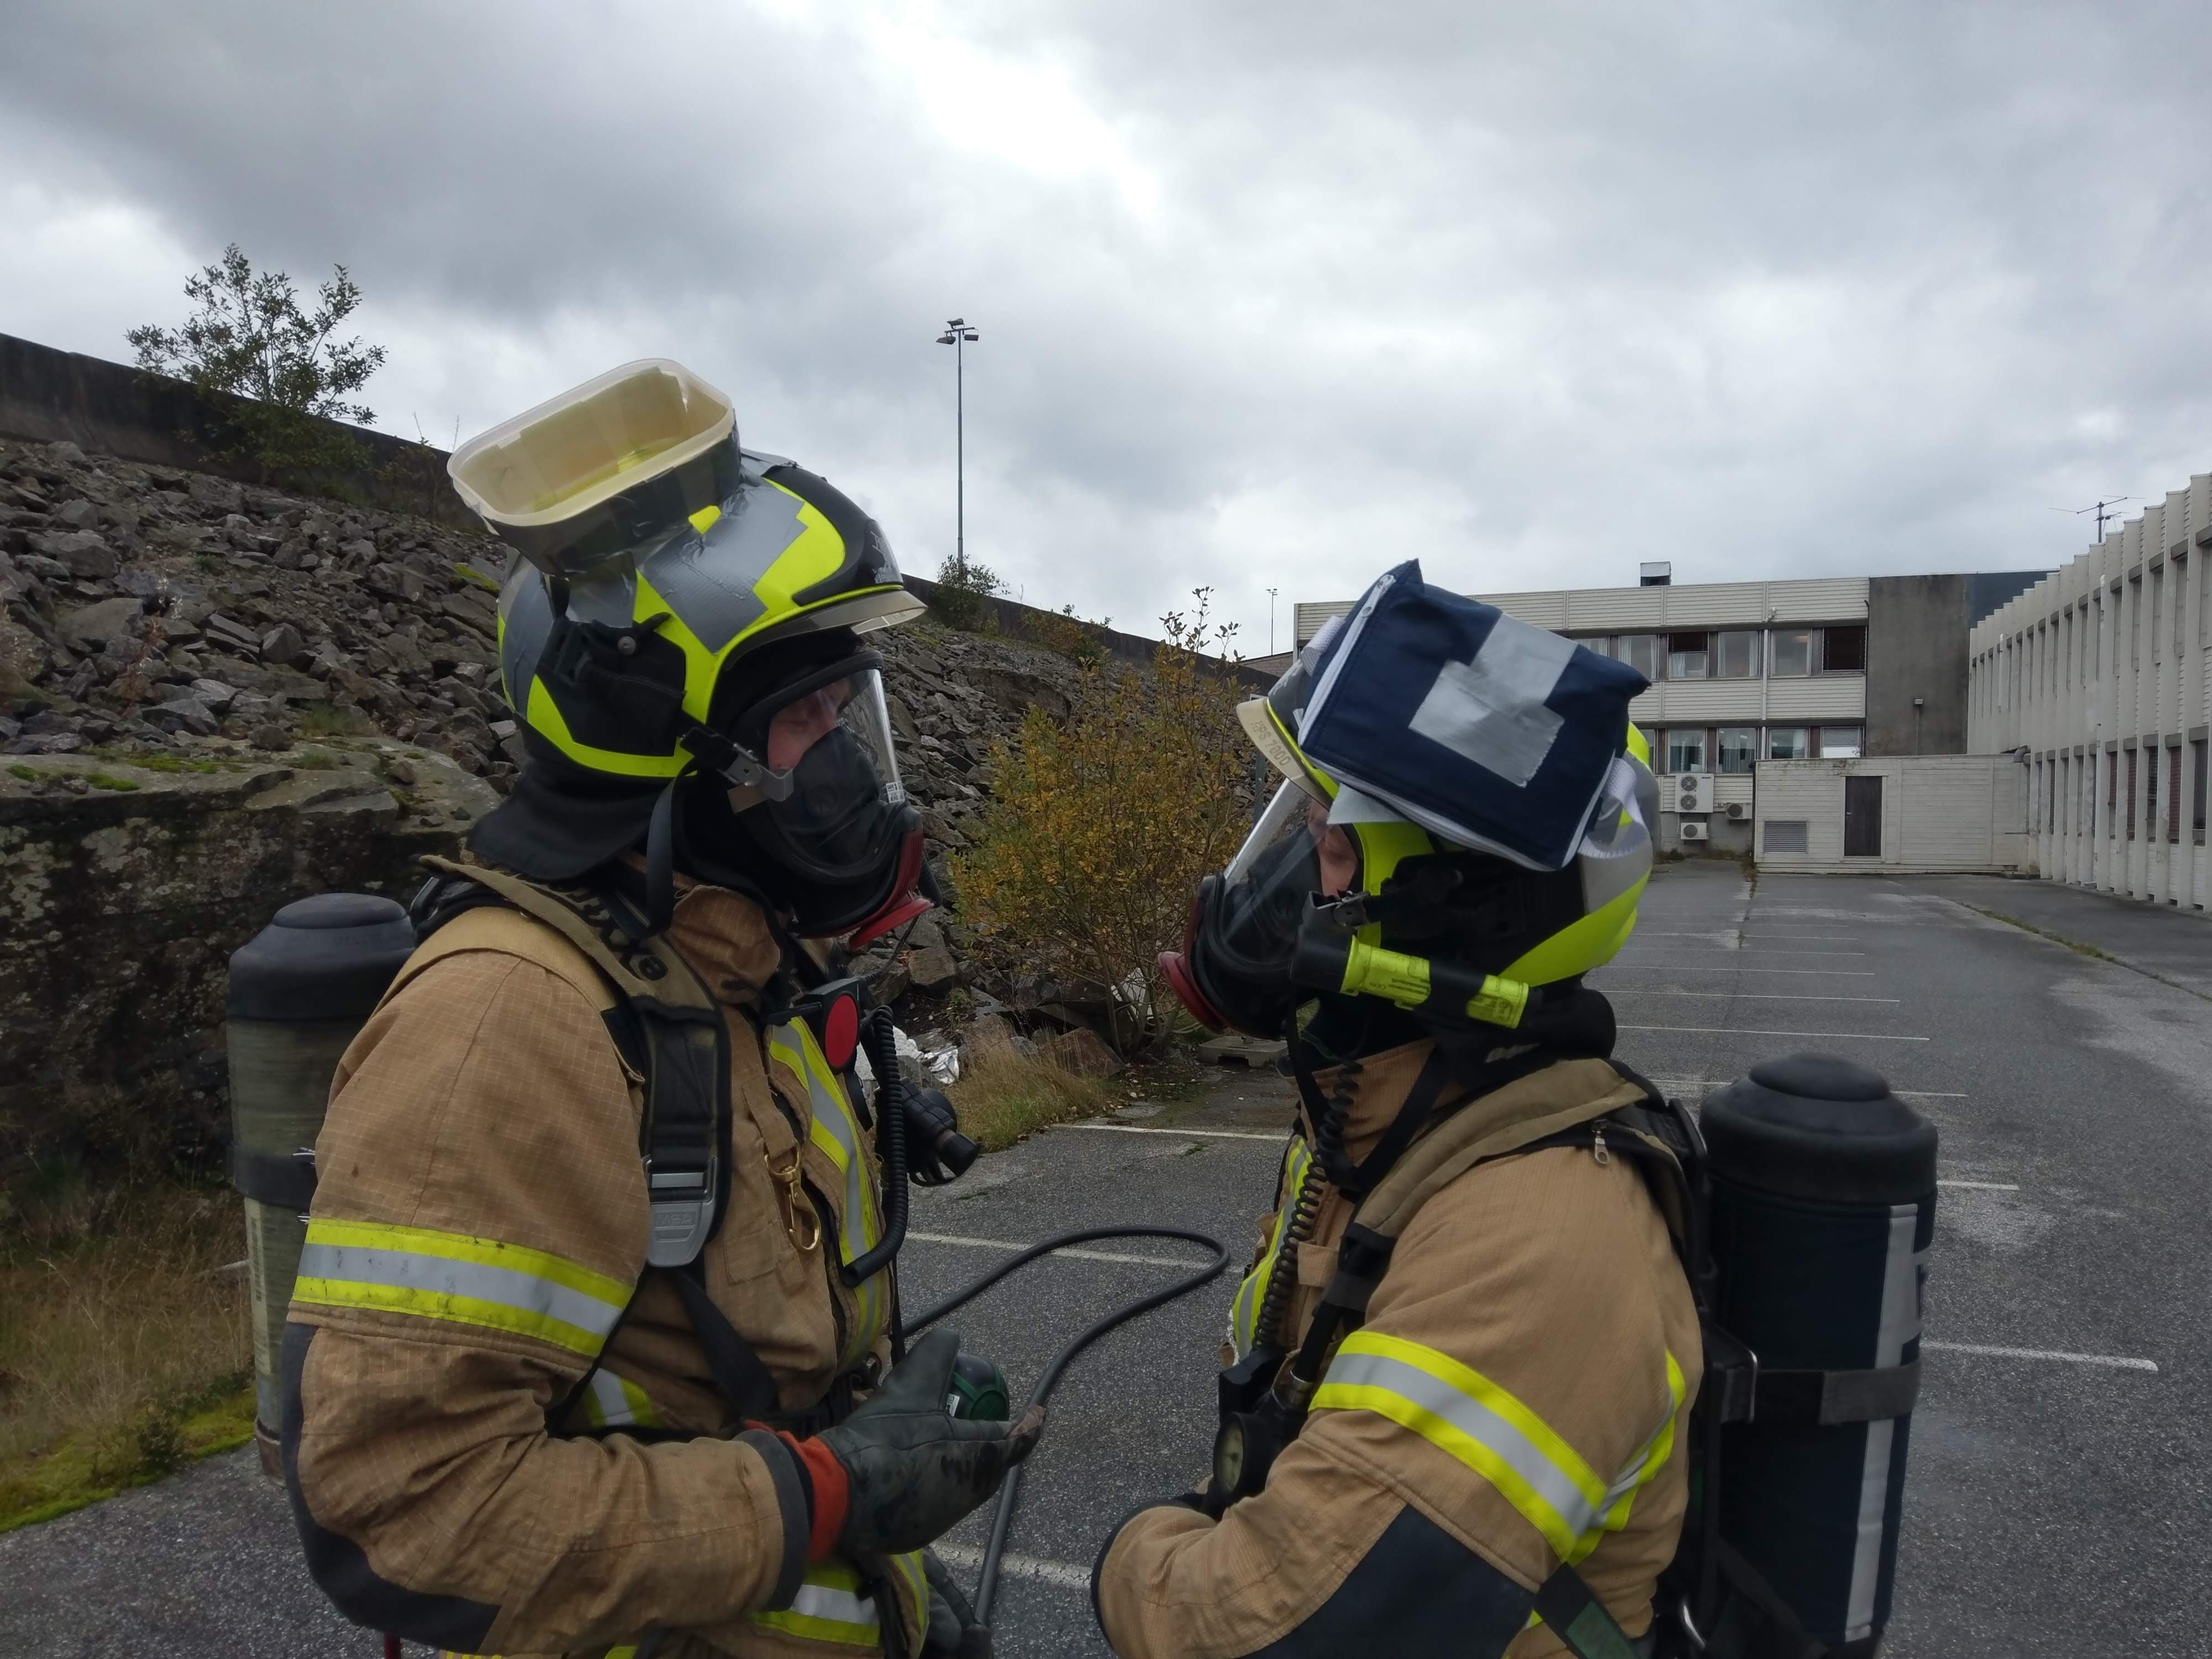
\includegraphics[width=\textwidth]{../fig/firefighters-with-helmet}
	\caption{Firefighters with smartphones mounted on their helmet}
	\label{fig:eval-firefighters}
\end{figure}

\section{Interview}

\section{System Usability Scale}

\section{Summary}

\end{document}
